\documentclass[SRC.tex]{subfiles}

\begin{document}
	
	For at kunne regne på, hvor effektiv en EuroDish er, så er det nødvendigt at opstille
	en matematisk model, som der kan regnes på. En sådan model tager afsæt i selve den del
	på EuroDishen, som omdanner solens energi til mekanisk energi, altså Stirlingmotoren. 
	
	\subsection{Analyse af en idealiseret Stirlingmotor}
	En idealiseret stirling motor er en model, som kan opstilles til en 
	Stirling motor, hvor de termodynamiske processorer sammensættes til en kredsproces. Da 
	de termodynamiske processorer er udledt af idealgaslignigen, så giver det 
	god mening, at en model opstillet med disse også vil være ideal. Den idealeliserede Stirling motor vil derfor ikke matche en realistisk Stirling Motor. Den idealiserede stirling motors \(pV\)-diagram kan ses på figur \ref{fig:stirlingcycle}
	
	\begin{figure}[h!]
		\centering
		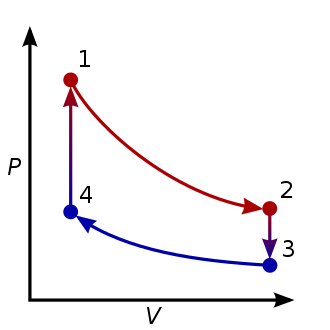
\includegraphics[width=0.4\linewidth]{Billeder/330px-Stirling_Cycle_color.svg}
		\caption{En idealiseret Stirling motos kredsproces indtegnet i et \(pV\)-diagram. Kilde: (Wikipedia, u.d.) }
		\label{fig:stirlingcycle}
	\end{figure}
	

	Hvor proces:
	\begin{enumerate}[]
		\item \quad \(1 \rightarrow 2\): er en isoterm ekspansion
		\item \quad \(2 \rightarrow 3\): er en iskor afkøling
		\item \quad \(3 \rightarrow 4\): er en isoterm kompression
		\item \quad \(4 \rightarrow 1\): er en isokor opvarmning
	\end{enumerate}
	(Holck og Kraaer, 2009)
	
	
	\subsubsection{Arbejde udført af en idealiseret Stirlingmotor}
	Nettoarbejdet for en idealiseret Stirling motor kan beregnes ved at finde arealet, der afgrænses
	af de termodynamiske processor  i \(pV\)-diagrammet. Der udføreres kun et arbejde ved 
	proces \(1\rightarrow2\), altså den isoterme ekspansion og ved den proces \(3 \rightarrow 4\), 
	den isoterme kompression. Arbejdet for en isoterm proces kan opfattes som araelet under den 
	afbillede graf i diagrammet. Derfor må nettoarbejdet være lig med forskellen på den øverste
	process og den nederste process, som rent matematisk kan udregnes som
	\begin{equation}
		A_{\text{netto}} = \int_{V_1}^{V_2} p \, dV - \int_{V_3}^{V_4} p \, dV 
		\label{eq:1}
	\end{equation}
	Selve arbejdet, som en isoterm udfører undervejs, kan findes ved at betrage ligning \eqref{eq:1},
	idealgasligningen, og huske at for en isoterm proces er temperaturen \(T\) konstant, samt stofmængden \(n\), da det er en kredsproces. Ud fra dette kan et udtryk for det udførte arbejde skrives som
	\begin{subequations}
		\begin{align}
		\int_{V_A}^{V_B} p \, dV &= \int_{V_A}^{V_B} \frac{nRT}{V} \, dV  = nRT \cdot 	\int_{V_A}^{V_B} \frac{1}{V}\, dV \\
		&= nRT \cdot \left[\ln V\right]_{V_A}^{V_B}  = nRT \cdot (\ln V_\text{B} - \ln V_\text{A})\\
		&=nRT \ln\left(\frac{V_B}{V_A}\right)
		\label{eq:workint}
		\end{align}
	\end{subequations}
	hvor \(V_{\text{B}}\) og \(V_{\text{A}}\) er henholdsvis slut- og startvolumenet. Fra trin b til c
	i ligning \eqref{eq:workint} anvendes, at \[\ln(A)-\ln(B) = \ln\left(\frac{A}{B}\right). \]
	Dette er den samme ligning, som blev introduceret i redegørelse, navnligt ligning \eqref{eq:10},
	den eneste forskel er fortegnet. I redegørelsen var det arbejdet, som omgivelserne skulle udføre
	på gassen, hvorimod det her er gassens arbejde. 
	Ved at substituere ligning \eqref{eq:workint} i ligning \eqref{eq:1}, så kan integralet for 
	nettoarbejdet evalueres på følgende vis
	\begin{equation}
		A_{\text{netto}} = nRT_H\ln\left(\frac{V_2}{V_1}\right)-nRT_L\ln\left(\frac{V_3}{V_4}\right)
	\end{equation}
	hvor subskriftene \(H\) og \(L\) denoterer henholdsvis den høje og lave temperatur i den isoterme
	proces. Ved at obsevere \(pV\)-diagrammet på figur \ref{fig:stirlingcycle}, så kan det ses at \(V_4 = V_1\) samt 
	at \(V_3 = V_2\), netop da to lodrette processor, er isokore processor, hvor volumenet holdes konstant. Herved kan ligningen omskrives til
	\begin{equation}
	A_{\text{netto}} = nRT_H\ln\left(\frac{V_2}{V_1}\right)-nRT_L\ln\left(\frac{V_2}{V_1}\right)
	\end{equation}
	Ved at faktorisere kan udtrykket skrives som
	\begin{equation}
		A_{\text{netto}}= nR\ln\left(\frac{V_2}{V_1}\right)\cdot (T_H - T_L)
		\label{eq:arbejde}
	\end{equation}
	Så arbejdet, som udføres på omgivelserne af en idealiseret Stirling motor kan beregnes ved anvendelse af ligning \eqref{eq:arbejde}.
	(Haywood) (Holck og Kraaer, 2009) 
	
	\subsubsection{Tilførsel af varme til systemet}
	Når den ideliserede cyklus når proces \(1 \rightarrow 2\), så sker der en 
	ekspansion, altså volumenet på gassen bliver større. Derfor skal der tilføres en hvis mængde 
	energi til gassen for at holde temperaturen i gassen konstant. Den mængde, \(Q\), som skal tilføres til gassen i kredsprocessen kan udledes ud fra ligning
	\begin{equation}
		Q_{\text{tilført}} = nRT_H\ln\left(\frac{V_2}{V_1}\right)
		\label{eq:varme}
	\end{equation}
	(Holck og Kraaer, 2009) 
	 
	\subsubsection{Nyttevirkning af en idealiseret Stirling motor}
	For en kraftvarmemaskine, som Stirling maskinen, er dens nyttevirkning defineret som forholdet mellem maskinens arbejde og den tilførte energi. Nyttevirkningen kan beregnes ved 
	\begin{equation}
		\eta = \frac{A_{\text{maskine}}}{Q_{\text{tilført}}}
		\label{eq:nyttevirkning}
	\end{equation}
	hvor \(A_{\text{maskine}}\) er maskinens arbejde og \(Q_{\text{tilført}}\) e varmen, der tilføres maskinen undervejs. For en idealiseret Stirling motor, så kan nyttevirkningen udregnes ved at indsææte ligning \eqref{eq:arbejde} og \eqref{eq:varme} i ligning \eqref{eq:nyttevirkning}, som resulterer i
	\begin{equation}
		\eta = \frac{nR\ln\left(\frac{V_2}{V_1}\right)\cdot (T_H - T_L)}{nRT_H\ln\left(\frac{V_2}{V_1}\right)} 
	\end{equation}
	Her kan det let ses, at \(nR\ln\left(\frac{V_2}{V_1}\right)\) i tæller og nævner vil udligne hinanden og så kan nyttevirkningen nu beregnes med
	\begin{equation}
		\eta = \frac{T_H-T_L}{T_H}
		\label{eq:nytte}
	\end{equation}
	Heraf kan det ses, at nyttevirkningen af en idealiseret stirling motor udelukkende afhænger af den højeste og laveste temperatur. Ved at omskrive ligning \eqref{eq:nytte} som følgende
	\begin{subequations}
		\begin{align}
			\eta &= \frac{T_H-T_L}{T_H} \\
			 	 &= \frac{T_H}{T_H}-\frac{T_L}{T_H} \\
			 	 &= 1 -\frac{T_L}{T_H}
		\end{align}
	\end{subequations}
	så kan det obseveres, at nyttevirkningen for en idealiseret stirling motor aldrig kan overstige 1.
	(Holck og Kraaer, 2009)​(Haywood) 
	\subsection{Beregning på modellen}
	Som det fremstod i det forrige, så kan nyttevirkningen for en idealiseret Stirling motor beregnes, hvis man kender den maksimale og minimale temperatur for gassen i kredsprocessen. I EuroDishen anvendes Stirling motoren, SOLO Stirling 161, der produceres af SOLO Kleinmotoren (Schiel og Laing, 2015) . I databladet for den anvendte Stirling motor fremgår det, at den maksimale driftstemperatur er \SI{650}{\celsius}, dog så fremgår den minimale temperatur ikke i databladet (SOLO Stirling) . Derfor tages der i det følgende afsæt i en anden Stirling motor, som har en maksimal temperatur på \SI{1054}{\kelvin} og en minimum på \SI{308}{\kelvin} (Granados, 2014) . 
	Ud fra disse data, så kan den teoretiske og idealiserede nyttevirkning for denne Stirling motor beregnes med ligning \eqref{eq:nytte}, som resulterer i
	\begin{equation}
		\eta_{\text{Stirling}} = \frac{\SI{1054}{\kelvin} - \SI{308}{\kelvin}}{\SI{1054}{\kelvin}} = 0.708 = \SI{70.8}{\percent}
	\end{equation}
	Det vil altså sige, at for al energi som tilføres til den idealiserede Stirling maskine, så vil en andel på \(\SI{70.8}{\percent}\) blive omdannet til mekanisk energi. For at udvide modellen til hele EuroDishen og ikke kun Stirling motoren, så kan der tilføres noget data, der gør modellen mere virkelighedsnær. For at en EuroDish kan generere el, så er der koblet en elgenereator på Stirling motoren, som omdanner det mekaniske energi til elektricitet. I det tidligere nævnte datablad, så fremgår virkningsgraden for den anvendte elgenerator, og er opgivet til at være \(\eta_{\text{gen}} = \SI{94}{\percent}\). Heraf kan den nyttevirkning fra tilført varmeenergi til elektrisk energi, genereret af generatoren, findes ved produktet af disse nyttevirkninger
	\begin{equation}
		\eta_{\text{q}\rightarrow\text{el}} =  \eta_{\text{stirling}} \cdot \eta_{\text{gen}} = 0.708 \cdot 0.94 = 0.665 = \SI{66.5}{\percent}
		\label{eq:31}
	\end{equation}
	Så for den energi, som tilføres til Stirling generatoren via sollys, vil en andel af \SI{67}{\percent} blive omdannet til elektrisk energi, der kan sendes ud til elnettet. Ligeledes kan der introduceres en faktor \(r\) om refleksiviteten af spejlene, som reflektere solen lys til Stirling Motoren i brændpunktet. Det er ikke alt lyset, som reflekteres af spejlene, hvilket ses ved at tilgå det tidligere nævnte datablad. Så kan det ses, at spejlene reflekterer \SI{97}{\percent} af det indgående sollys (Schiel og Laing, 2015) . Det reflekterede sollys modtages af en såkaldt 'reciever', som sidder på Stirling motoren og overfører varmen dertil. Ved denne introduceres også et tab af energi, nemlig da den har en nyttevirkning, \(\eta_{\text{reciever}} = \SI{90}{\percent}\). Så kan refleksivitens fakor, \(r\) og nyttevirkningen af recieveren ganges på ligning \eqref{eq:31}. Heraf fås en mere præcis model af EuroDishens nyttevirknig.
	\begin{equation}
		\eta_{\text{eurodish}} = \eta_{\text{q}\rightarrow\text{el}} \cdot r \cdot \eta_{\text{reciever}}  = 0.665 \cdot 0.97 \cdot 0.90 = 0.58 = \SI{58}{\percent}
		\label{eq:nyt}
	\end{equation} 
	Så af al ingående solenergi, så vil, efter denne model, \SI{58}{\percent} af energien blive omdannet til elektricitet. 
	\subsection{Sammenligning}
	De største indenfor anvendelsen af solenergi er solcellerne. Mono-krystallinske solceller har en nyttevirkning på 22-\SI{27}{\percent} (Vourvoulias, 2021).
	Den opstillede model for EuroDishen fremsætter, at den har en nyttevirkning på \SI{58}{\percent} 
	og dermed omdanner den lidt over dobbelt så meget, som solcellerne eller rettere sagt solpanelerne og dermed en EuroDish modellen præsenteret i dette projekt mere effektiv end solpanelerne. 

\end{document}